\documentclass{acmsiggraph}
\usepackage[english]{babel}
\usepackage[T1]{fontenc}
\usepackage[latin1]{inputenc}
\usepackage{float, enumitem, footnote, multirow}
\usepackage[font=scriptsize,labelfont=bf, justification=centering, format=hang]{caption}
\DeclareCaptionFont{tiny}{\tiny}

\usepackage[font=tiny]{subfig}
\usepackage{amsmath, amsthm, amssymb, bbm}
\usepackage[ruled,vlined]{algorithm2e}
\usepackage{hyperref}
\usepackage{microtype}
\usepackage{lmodern}
\usepackage{listings}
\lstset{
	basicstyle=\footnotesize
}
\graphicspath{{../figures/}}
\DeclareMathOperator\sign{sign}

\newcommand\mycommfont[1]{\footnotesize\ttfamily{#1}}
\SetCommentSty{mycommfont}
\newcommand{\R}{\mathbb{R}}
\newcommand{\1}{\mathbbm{1}}
\DeclareMathOperator\sig{sigmoid}


%-----------------------
% TIKZ
% -----------------------
    \usepackage{tikz}
    \usetikzlibrary{arrows,positioning}
    \tikzstyle{circ}=[draw, circle, fill=white, align=center, inner sep=1,outer sep=0]



\title{Machine Learning for Computer Vision\\ {\large [MVA 2015/2016]}\\
\vspace{10pt}
Final assignment}

\author{Maha ELBAYAD
%\\ \texttt{maha.elbayad@student.ecp.fr}}
}
\pdfauthor{Maha ELBAYAD}
\newcommand{\E}{\mathbb{E}}
\begin{document}
\maketitle
\section{Detector training}
	We trained different classifiers: Linear regression, L2-logistic regression (c.f. assignment 1), linear SVM and RBF-SVM (c.f. assignement 2) to detect particular points of a facial image namely the left eye, right eye, left mouth, right mouth and nose. Each of these classifier is either trained on SIFT features or CNN features extracted with an Alexnet pre-trained network\footnote{http://www.vlfeat.org/matconvnet/models/beta16/imagenet-caffe-alex.mat} shown in figure (\ref{model}) where the features are either the outpout of the relu2 layer denoted \texttt{CNN2} or that of the relu5 layer denoted \texttt{CNN5}. 
	\begin{figure}[H]
	\centering
	\includegraphics[width=19cm]{part1/model}
	\caption{\label{model}Alexnet architecture}
	\end{figure}

	If needed we choose the classifier's optimal parameters with cross-validation (5-folds).

	\subsection{Precision recall curves:}
		\begin{figure}[H]
		\centering
		\subfloat[Right eye]{\includegraphics[width=3cm]{"part1/Features_SIFT_Part_Right eye_pr"}}
		\subfloat[Left eye]{\includegraphics[width=3cm]{"part1/Features_SIFT_Part_Left eye_pr"}}
		\subfloat[Left mouth]{\includegraphics[width=3cm]{"part1/Features_SIFT_Part_Left mouth_pr"}}
		\subfloat[Right mouth]{\includegraphics[width=3cm]{"part1/Features_SIFT_Part_Right mouth_pr"}}
		\subfloat[Nose]{\includegraphics[width=3cm]{"part1/Features_SIFT_Part_Nose_pr"}}
		\caption{SIFT features}
		\end{figure}
		\begin{figure}[H]
		\centering
		\subfloat[Right eye]{\includegraphics[width=3cm]{"part1/Features_CNN2_Part_Right eye_pr"}}
		\subfloat[Left eye]{\includegraphics[width=3cm]{"part1/Features_CNN2_Part_Left eye_pr"}}
		\subfloat[Left mouth]{\includegraphics[width=3cm]{"part1/Features_CNN2_Part_Left mouth_pr"}}
		\subfloat[Right mouth]{\includegraphics[width=3cm]{"part1/Features_CNN2_Part_Right mouth_pr"}}
		\subfloat[Nose]{\includegraphics[width=3cm]{"part1/Features_CNN2_Part_Nose_pr"}}
		\caption{CNN2 features}
		\end{figure}
		\begin{figure}[H]
		\centering
		\subfloat[Right eye]{\includegraphics[width=3cm]{"part1/Features_CNN5_Part_Right eye_pr"}}
		\subfloat[Left eye]{\includegraphics[width=3cm]{"part1/Features_CNN5_Part_Left eye_pr"}}
		\subfloat[Left mouth]{\includegraphics[width=3cm]{"part1/Features_CNN5_Part_Left mouth_pr"}}
		\subfloat[Right mouth]{\includegraphics[width=3cm]{"part1/Features_CNN5_Part_Right mouth_pr"}}
		\subfloat[Nose]{\includegraphics[width=3cm]{"part1/Features_CNN5_Part_Nose_pr"}}
		\caption{CNN5 features}
		\end{figure}

	\subsection{SIFT features - Dense scores}
		For two samples from different categories we show the dense scores of each classifier.
		\begin{figure}[H]
		\centering
		\subfloat[Face]{\includegraphics[height=2.1cm]{part1/human}}
		\hspace{5pt}\subfloat[Background]{\includegraphics[height=2.1cm]{part1/bg}}
		\caption{Input images}
		\end{figure}
		\begin{figure}[H]
		\centering
		\subfloat[LR (1)]{\includegraphics[height=2.1cm]{"part1/Features_SIFT_Part_Right eye_Classifier_Linear_dense_1"}}
		\hspace{1pt}\subfloat[LR (0)]{\includegraphics[height=2.1cm]{"part1/Features_SIFT_Part_Right eye_Classifier_Linear_dense_0"}}
		\hspace{1pt}\subfloat[Logistic (1)]{\includegraphics[height=2.1cm]{"part1/Features_SIFT_Part_Right eye_Classifier_Logistic_dense_1"}}
		\hspace{1pt}\subfloat[Logistic (0)]{\includegraphics[height=2.1cm]{"part1/Features_SIFT_Part_Right eye_Classifier_Logistic_dense_0"}}
		\hspace{1pt}\subfloat[SVM (1)]{\includegraphics[height=2.1cm]{"part1/Features_SIFT_Part_Right eye_Classifier_SVM_dense_1"}}
		\hspace{1pt}\subfloat[SVM (0)]{\includegraphics[height=2.1cm]{"part1/Features_SIFT_Part_Right eye_Classifier_SVM_dense_0"}}
		\hspace{1pt}\subfloat[SVM-RBF (1)]{\includegraphics[height=2.1cm]{"part1/Features_SIFT_Part_Right eye_Classifier_SVM-RBF_dense_1"}}
		\hspace{1pt}\subfloat[SVM-RBF (0)]{\includegraphics[height=2.1cm]{"part1/Features_SIFT_Part_Right eye_Classifier_SVM-RBF_dense_0"}}
		\caption{Right eye}
		\end{figure}

		\begin{figure}[H]
		\centering
		\subfloat[LR (1)]{\includegraphics[height=2.1cm]{"part1/Features_SIFT_Part_Left eye_Classifier_Linear_dense_1"}}
		\hspace{1pt}\subfloat[LR (0)]{\includegraphics[height=2.1cm]{"part1/Features_SIFT_Part_Left eye_Classifier_Linear_dense_0"}}
		\hspace{1pt}\subfloat[Logistic (1)]{\includegraphics[height=2.1cm]{"part1/Features_SIFT_Part_Left eye_Classifier_Logistic_dense_1"}}
		\hspace{1pt}\subfloat[Logistic (0)]{\includegraphics[height=2.1cm]{"part1/Features_SIFT_Part_Left eye_Classifier_Logistic_dense_0"}}
		\hspace{1pt}\subfloat[SVM (1)]{\includegraphics[height=2.1cm]{"part1/Features_SIFT_Part_Left eye_Classifier_SVM_dense_1"}}
		\hspace{1pt}\subfloat[SVM (0)]{\includegraphics[height=2.1cm]{"part1/Features_SIFT_Part_Left eye_Classifier_SVM_dense_0"}}
		\hspace{1pt}\subfloat[SVM-RBF (1)]{\includegraphics[height=2.1cm]{"part1/Features_SIFT_Part_Left eye_Classifier_SVM-RBF_dense_1"}}
		\hspace{1pt}\subfloat[SVM-RBF (0)]{\includegraphics[height=2.1cm]{"part1/Features_SIFT_Part_Left eye_Classifier_SVM-RBF_dense_0"}}
		\caption{Left eye}
		\end{figure}

		\begin{figure}[H]
		\centering
		\subfloat[LR (1)]{\includegraphics[height=2.1cm]{"part1/Features_SIFT_Part_Left mouth_Classifier_Linear_dense_1"}}
		\hspace{1pt}\subfloat[LR (0)]{\includegraphics[height=2.1cm]{"part1/Features_SIFT_Part_Left mouth_Classifier_Linear_dense_0"}}
		\hspace{1pt}\subfloat[Logistic (1)]{\includegraphics[height=2.1cm]{"part1/Features_SIFT_Part_Left mouth_Classifier_Logistic_dense_1"}}
		\hspace{1pt}\subfloat[Logistic (0)]{\includegraphics[height=2.1cm]{"part1/Features_SIFT_Part_Left mouth_Classifier_Logistic_dense_0"}}
		\hspace{1pt}\subfloat[SVM (1)]{\includegraphics[height=2.1cm]{"part1/Features_SIFT_Part_Left mouth_Classifier_SVM_dense_1"}}
		\hspace{1pt}\subfloat[SVM (0)]{\includegraphics[height=2.1cm]{"part1/Features_SIFT_Part_Left mouth_Classifier_SVM_dense_0"}}
		\hspace{1pt}\subfloat[SVM-RBF (1)]{\includegraphics[height=2.1cm]{"part1/Features_SIFT_Part_Left mouth_Classifier_SVM-RBF_dense_1"}}
		\hspace{1pt}\subfloat[SVM-RBF (0)]{\includegraphics[height=2.1cm]{"part1/Features_SIFT_Part_Left mouth_Classifier_SVM-RBF_dense_0"}}
		\caption{Left mouth}
		\end{figure}

		\begin{figure}[H]
		\centering
		\subfloat[LR (1)]{\includegraphics[height=2.1cm]{"part1/Features_SIFT_Part_Right mouth_Classifier_Linear_dense_1"}}
		\hspace{1pt}\subfloat[LR (0)]{\includegraphics[height=2.1cm]{"part1/Features_SIFT_Part_Right mouth_Classifier_Linear_dense_0"}}
		\hspace{1pt}\subfloat[Logistic (1)]{\includegraphics[height=2.1cm]{"part1/Features_SIFT_Part_Right mouth_Classifier_Logistic_dense_1"}}
		\hspace{1pt}\subfloat[Logistic (0)]{\includegraphics[height=2.1cm]{"part1/Features_SIFT_Part_Right mouth_Classifier_Logistic_dense_0"}}
		\hspace{1pt}\subfloat[SVM (1)]{\includegraphics[height=2.1cm]{"part1/Features_SIFT_Part_Right mouth_Classifier_SVM_dense_1"}}
		\hspace{1pt}\subfloat[SVM (0)]{\includegraphics[height=2.1cm]{"part1/Features_SIFT_Part_Right mouth_Classifier_SVM_dense_0"}}
		\hspace{1pt}\subfloat[SVM-RBF (1)]{\includegraphics[height=2.1cm]{"part1/Features_SIFT_Part_Right mouth_Classifier_SVM-RBF_dense_1"}}
		\hspace{1pt}\subfloat[SVM-RBF (0)]{\includegraphics[height=2.1cm]{"part1/Features_SIFT_Part_Right mouth_Classifier_SVM-RBF_dense_0"}}
		\caption{Right mouth}
		\end{figure}

		\begin{figure}[H]
		\centering
		\subfloat[LR (1)]{\includegraphics[height=2.1cm]{"part1/Features_SIFT_Part_Nose_Classifier_Linear_dense_1"}}
		\hspace{1pt}\subfloat[LR (0)]{\includegraphics[height=2.1cm]{"part1/Features_SIFT_Part_Nose_Classifier_Linear_dense_0"}}
		\hspace{1pt}\subfloat[Logistic (1)]{\includegraphics[height=2.1cm]{"part1/Features_SIFT_Part_Nose_Classifier_Logistic_dense_1"}}
		\hspace{1pt}\subfloat[Logistic (0)]{\includegraphics[height=2.1cm]{"part1/Features_SIFT_Part_Nose_Classifier_Logistic_dense_0"}}
		\hspace{1pt}\subfloat[SVM (1)]{\includegraphics[height=2.1cm]{"part1/Features_SIFT_Part_Nose_Classifier_SVM_dense_1"}}
		\hspace{1pt}\subfloat[SVM (0)]{\includegraphics[height=2.1cm]{"part1/Features_SIFT_Part_Nose_Classifier_SVM_dense_0"}}
		\hspace{1pt}\subfloat[SVM-RBF (1)]{\includegraphics[height=2.1cm]{"part1/Features_SIFT_Part_Nose_Classifier_SVM-RBF_dense_1"}}
		\hspace{1pt}\subfloat[SVM-RBF (0)]{\includegraphics[height=2.1cm]{"part1/Features_SIFT_Part_Nose_Classifier_SVM-RBF_dense_0"}}
		\caption{Nose}
		\end{figure}

	\subsection{CNN2 features - Dense scores}
		\begin{figure}[H]
		\centering
		\subfloat[LR (1)]{\includegraphics[height=2.1cm]{"part1/Features_CNN2_Part_Right eye_Classifier_Linear_dense_1"}}
		\hspace{1pt}\subfloat[LR (0)]{\includegraphics[height=2.1cm]{"part1/Features_CNN2_Part_Right eye_Classifier_Linear_dense_0"}}
		\hspace{1pt}\subfloat[Logistic (1)]{\includegraphics[height=2.1cm]{"part1/Features_CNN2_Part_Right eye_Classifier_Logistic_dense_1"}}
		\hspace{1pt}\subfloat[Logistic (0)]{\includegraphics[height=2.1cm]{"part1/Features_CNN2_Part_Right eye_Classifier_Logistic_dense_0"}}
		\hspace{1pt}\subfloat[SVM (1)]{\includegraphics[height=2.1cm]{"part1/Features_CNN2_Part_Right eye_Classifier_SVM_dense_1"}}
		\hspace{1pt}\subfloat[SVM (0)]{\includegraphics[height=2.1cm]{"part1/Features_CNN2_Part_Right eye_Classifier_SVM_dense_0"}}
		\hspace{1pt}\subfloat[SVM-RBF (1)]{\includegraphics[height=2.1cm]{"part1/Features_CNN2_Part_Right eye_Classifier_SVM-RBF_dense_1"}}
		\hspace{1pt}\subfloat[SVM-RBF (0)]{\includegraphics[height=2.1cm]{"part1/Features_CNN2_Part_Right eye_Classifier_SVM-RBF_dense_0"}}
		\caption{Right eye}
		\end{figure}

		\begin{figure}[H]
		\centering
		\subfloat[LR (1)]{\includegraphics[height=2.1cm]{"part1/Features_CNN2_Part_Left eye_Classifier_Linear_dense_1"}}
		\hspace{1pt}\subfloat[LR (0)]{\includegraphics[height=2.1cm]{"part1/Features_CNN2_Part_Left eye_Classifier_Linear_dense_0"}}
		\hspace{1pt}\subfloat[Logistic (1)]{\includegraphics[height=2.1cm]{"part1/Features_CNN2_Part_Left eye_Classifier_Logistic_dense_1"}}
		\hspace{1pt}\subfloat[Logistic (0)]{\includegraphics[height=2.1cm]{"part1/Features_CNN2_Part_Left eye_Classifier_Logistic_dense_0"}}
		\hspace{1pt}\subfloat[SVM (1)]{\includegraphics[height=2.1cm]{"part1/Features_CNN2_Part_Left eye_Classifier_SVM_dense_1"}}
		\hspace{1pt}\subfloat[SVM (0)]{\includegraphics[height=2.1cm]{"part1/Features_CNN2_Part_Left eye_Classifier_SVM_dense_0"}}
		\hspace{1pt}\subfloat[SVM-RBF (1)]{\includegraphics[height=2.1cm]{"part1/Features_CNN2_Part_Left eye_Classifier_SVM-RBF_dense_1"}}
		\hspace{1pt}\subfloat[SVM-RBF (0)]{\includegraphics[height=2.1cm]{"part1/Features_CNN2_Part_Left eye_Classifier_SVM-RBF_dense_0"}}
		\caption{Left eye}
		\end{figure}

		\begin{figure}[H]
		\centering
		\subfloat[LR (1)]{\includegraphics[height=2.1cm]{"part1/Features_CNN2_Part_Left mouth_Classifier_Linear_dense_1"}}
		\hspace{1pt}\subfloat[LR (0)]{\includegraphics[height=2.1cm]{"part1/Features_CNN2_Part_Left mouth_Classifier_Linear_dense_0"}}
		\hspace{1pt}\subfloat[Logistic (1)]{\includegraphics[height=2.1cm]{"part1/Features_CNN2_Part_Left mouth_Classifier_Logistic_dense_1"}}
		\hspace{1pt}\subfloat[Logistic (0)]{\includegraphics[height=2.1cm]{"part1/Features_CNN2_Part_Left mouth_Classifier_Logistic_dense_0"}}
		\hspace{1pt}\subfloat[SVM (1)]{\includegraphics[height=2.1cm]{"part1/Features_CNN2_Part_Left mouth_Classifier_SVM_dense_1"}}
		\hspace{1pt}\subfloat[SVM (0)]{\includegraphics[height=2.1cm]{"part1/Features_CNN2_Part_Left mouth_Classifier_SVM_dense_0"}}
		\hspace{1pt}\subfloat[SVM-RBF (1)]{\includegraphics[height=2.1cm]{"part1/Features_CNN2_Part_Left mouth_Classifier_SVM-RBF_dense_1"}}
		\hspace{1pt}\subfloat[SVM-RBF (0)]{\includegraphics[height=2.1cm]{"part1/Features_CNN2_Part_Left mouth_Classifier_SVM-RBF_dense_0"}}
		\caption{Left mouth}
		\end{figure}

		\begin{figure}[H]
		\centering
		\subfloat[LR (1)]{\includegraphics[height=2.1cm]{"part1/Features_CNN2_Part_Right mouth_Classifier_Linear_dense_1"}}
		\hspace{1pt}\subfloat[LR (0)]{\includegraphics[height=2.1cm]{"part1/Features_CNN2_Part_Right mouth_Classifier_Linear_dense_0"}}
		\hspace{1pt}\subfloat[Logistic (1)]{\includegraphics[height=2.1cm]{"part1/Features_CNN2_Part_Right mouth_Classifier_Logistic_dense_1"}}
		\hspace{1pt}\subfloat[Logistic (0)]{\includegraphics[height=2.1cm]{"part1/Features_CNN2_Part_Right mouth_Classifier_Logistic_dense_0"}}
		\hspace{1pt}\subfloat[SVM (1)]{\includegraphics[height=2.1cm]{"part1/Features_CNN2_Part_Right mouth_Classifier_SVM_dense_1"}}
		\hspace{1pt}\subfloat[SVM (0)]{\includegraphics[height=2.1cm]{"part1/Features_CNN2_Part_Right mouth_Classifier_SVM_dense_0"}}
		\hspace{1pt}\subfloat[SVM-RBF (1)]{\includegraphics[height=2.1cm]{"part1/Features_CNN2_Part_Right mouth_Classifier_SVM-RBF_dense_1"}}
		\hspace{1pt}\subfloat[SVM-RBF (0)]{\includegraphics[height=2.1cm]{"part1/Features_CNN2_Part_Right mouth_Classifier_SVM-RBF_dense_0"}}
		\caption{Right mouth}
		\end{figure}

		\begin{figure}[H]
		\centering
		\subfloat[LR (1)]{\includegraphics[height=2.1cm]{"part1/Features_CNN2_Part_Nose_Classifier_Linear_dense_1"}}
		\hspace{1pt}\subfloat[LR (0)]{\includegraphics[height=2.1cm]{"part1/Features_CNN2_Part_Nose_Classifier_Linear_dense_0"}}
		\hspace{1pt}\subfloat[Logistic (1)]{\includegraphics[height=2.1cm]{"part1/Features_CNN2_Part_Nose_Classifier_Logistic_dense_1"}}
		\hspace{1pt}\subfloat[Logistic (0)]{\includegraphics[height=2.1cm]{"part1/Features_CNN2_Part_Nose_Classifier_Logistic_dense_0"}}
		\hspace{1pt}\subfloat[SVM (1)]{\includegraphics[height=2.1cm]{"part1/Features_CNN2_Part_Nose_Classifier_SVM_dense_1"}}
		\hspace{1pt}\subfloat[SVM (0)]{\includegraphics[height=2.1cm]{"part1/Features_CNN2_Part_Nose_Classifier_SVM_dense_0"}}
		\hspace{1pt}\subfloat[SVM-RBF (1)]{\includegraphics[height=2.1cm]{"part1/Features_CNN2_Part_Nose_Classifier_SVM-RBF_dense_1"}}
		\hspace{1pt}\subfloat[SVM-RBF (0)]{\includegraphics[height=2.1cm]{"part1/Features_SIFT_Part_Nose_Classifier_SVM-RBF_dense_0"}}
		\caption{Nose}
		\end{figure}

	\subsection{CNN5 features - Dense scores}
		\begin{figure}[H]
		\centering
		\subfloat[LR (1)]{\includegraphics[height=2.1cm]{"part1/Features_CNN5_Part_Right eye_Classifier_Linear_dense_1"}}
		\hspace{1pt}\subfloat[LR (0)]{\includegraphics[height=2.1cm]{"part1/Features_CNN5_Part_Right eye_Classifier_Linear_dense_0"}}
		\hspace{1pt}\subfloat[Logistic (1)]{\includegraphics[height=2.1cm]{"part1/Features_CNN5_Part_Right eye_Classifier_Logistic_dense_1"}}
		\hspace{1pt}\subfloat[Logistic (0)]{\includegraphics[height=2.1cm]{"part1/Features_CNN5_Part_Right eye_Classifier_Logistic_dense_0"}}
		\hspace{1pt}\subfloat[SVM (1)]{\includegraphics[height=2.1cm]{"part1/Features_CNN5_Part_Right eye_Classifier_SVM_dense_1"}}
		\hspace{1pt}\subfloat[SVM (0)]{\includegraphics[height=2.1cm]{"part1/Features_CNN5_Part_Right eye_Classifier_SVM_dense_0"}}
		\hspace{1pt}\subfloat[SVM-RBF (1)]{\includegraphics[height=2.1cm]{"part1/Features_CNN5_Part_Right eye_Classifier_SVM-RBF_dense_1"}}
		\hspace{1pt}\subfloat[SVM-RBF (0)]{\includegraphics[height=2.1cm]{"part1/Features_CNN5_Part_Right eye_Classifier_SVM-RBF_dense_0"}}
		\caption{Right eye}
		\end{figure}

		\begin{figure}[H]
		\centering
		\subfloat[LR (1)]{\includegraphics[height=2.1cm]{"part1/Features_CNN5_Part_Left eye_Classifier_Linear_dense_1"}}
		\hspace{1pt}\subfloat[LR (0)]{\includegraphics[height=2.1cm]{"part1/Features_CNN5_Part_Left eye_Classifier_Linear_dense_0"}}
		\hspace{1pt}\subfloat[Logistic (1)]{\includegraphics[height=2.1cm]{"part1/Features_CNN5_Part_Left eye_Classifier_Logistic_dense_1"}}
		\hspace{1pt}\subfloat[Logistic (0)]{\includegraphics[height=2.1cm]{"part1/Features_CNN5_Part_Left eye_Classifier_Logistic_dense_0"}}
		\hspace{1pt}\subfloat[SVM (1)]{\includegraphics[height=2.1cm]{"part1/Features_CNN5_Part_Left eye_Classifier_SVM_dense_1"}}
		\hspace{1pt}\subfloat[SVM (0)]{\includegraphics[height=2.1cm]{"part1/Features_CNN5_Part_Left eye_Classifier_SVM_dense_0"}}
		\hspace{1pt}\subfloat[SVM-RBF (1)]{\includegraphics[height=2.1cm]{"part1/Features_CNN5_Part_Left eye_Classifier_SVM-RBF_dense_1"}}
		\hspace{1pt}\subfloat[SVM-RBF (0)]{\includegraphics[height=2.1cm]{"part1/Features_CNN5_Part_Left eye_Classifier_SVM-RBF_dense_0"}}
		\caption{Left eye}
		\end{figure}

		\begin{figure}[H]
		\centering
		\subfloat[LR (1)]{\includegraphics[height=2.1cm]{"part1/Features_CNN5_Part_Left mouth_Classifier_Linear_dense_1"}}
		\hspace{1pt}\subfloat[LR (0)]{\includegraphics[height=2.1cm]{"part1/Features_CNN5_Part_Left mouth_Classifier_Linear_dense_0"}}
		\hspace{1pt}\subfloat[Logistic (1)]{\includegraphics[height=2.1cm]{"part1/Features_CNN5_Part_Left mouth_Classifier_Logistic_dense_1"}}
		\hspace{1pt}\subfloat[Logistic (0)]{\includegraphics[height=2.1cm]{"part1/Features_CNN5_Part_Left mouth_Classifier_Logistic_dense_0"}}
		\hspace{1pt}\subfloat[SVM (1)]{\includegraphics[height=2.1cm]{"part1/Features_CNN5_Part_Left mouth_Classifier_SVM_dense_1"}}
		\hspace{1pt}\subfloat[SVM (0)]{\includegraphics[height=2.1cm]{"part1/Features_CNN5_Part_Left mouth_Classifier_SVM_dense_0"}}
		\hspace{1pt}\subfloat[SVM-RBF (1)]{\includegraphics[height=2.1cm]{"part1/Features_CNN5_Part_Left mouth_Classifier_SVM-RBF_dense_1"}}
		\hspace{1pt}\subfloat[SVM-RBF (0)]{\includegraphics[height=2.1cm]{"part1/Features_CNN5_Part_Left mouth_Classifier_SVM-RBF_dense_0"}}
		\caption{Left mouth}
		\end{figure}

		\begin{figure}[H]
		\centering
		\subfloat[LR (1)]{\includegraphics[height=2.1cm]{"part1/Features_CNN5_Part_Right mouth_Classifier_Linear_dense_1"}}
		\hspace{1pt}\subfloat[LR (0)]{\includegraphics[height=2.1cm]{"part1/Features_CNN5_Part_Right mouth_Classifier_Linear_dense_0"}}
		\hspace{1pt}\subfloat[Logistic (1)]{\includegraphics[height=2.1cm]{"part1/Features_CNN5_Part_Right mouth_Classifier_Logistic_dense_1"}}
		\hspace{1pt}\subfloat[Logistic (0)]{\includegraphics[height=2.1cm]{"part1/Features_CNN5_Part_Right mouth_Classifier_Logistic_dense_0"}}
		\hspace{1pt}\subfloat[SVM (1)]{\includegraphics[height=2.1cm]{"part1/Features_CNN5_Part_Right mouth_Classifier_SVM_dense_1"}}
		\hspace{1pt}\subfloat[SVM (0)]{\includegraphics[height=2.1cm]{"part1/Features_CNN5_Part_Right mouth_Classifier_SVM_dense_0"}}
		\hspace{1pt}\subfloat[SVM-RBF (1)]{\includegraphics[height=2.1cm]{"part1/Features_CNN5_Part_Right mouth_Classifier_SVM-RBF_dense_1"}}
		\hspace{1pt}\subfloat[SVM-RBF (0)]{\includegraphics[height=2.1cm]{"part1/Features_CNN5_Part_Right mouth_Classifier_SVM-RBF_dense_0"}}
		\caption{Right mouth}
		\end{figure}

		\begin{figure}[H]
		\centering
		\subfloat[LR (1)]{\includegraphics[height=2.1cm]{"part1/Features_CNN5_Part_Nose_Classifier_Linear_dense_1"}}
		\hspace{1pt}\subfloat[LR (0)]{\includegraphics[height=2.1cm]{"part1/Features_CNN5_Part_Nose_Classifier_Linear_dense_0"}}
		\hspace{1pt}\subfloat[Logistic (1)]{\includegraphics[height=2.1cm]{"part1/Features_CNN5_Part_Nose_Classifier_Logistic_dense_1"}}
		\hspace{1pt}\subfloat[Logistic (0)]{\includegraphics[height=2.1cm]{"part1/Features_CNN5_Part_Nose_Classifier_Logistic_dense_0"}}
		\hspace{1pt}\subfloat[SVM (1)]{\includegraphics[height=2.1cm]{"part1/Features_CNN5_Part_Nose_Classifier_SVM_dense_1"}}
		\hspace{1pt}\subfloat[SVM (0)]{\includegraphics[height=2.1cm]{"part1/Features_CNN5_Part_Nose_Classifier_SVM_dense_0"}}
		\hspace{1pt}\subfloat[SVM-RBF (1)]{\includegraphics[height=2.1cm]{"part1/Features_CNN5_Part_Nose_Classifier_SVM-RBF_dense_1"}}
		\hspace{1pt}\subfloat[SVM-RBF (0)]{\includegraphics[height=2.1cm]{"part1/Features_SIFT_Part_Nose_Classifier_SVM-RBF_dense_0"}}
		\caption{Nose}
		\end{figure}

\section{Combination: Max-product for DPM detection}
	\begin{figure}[H]
		\centering
		\resizebox{0.3\textwidth}{!}{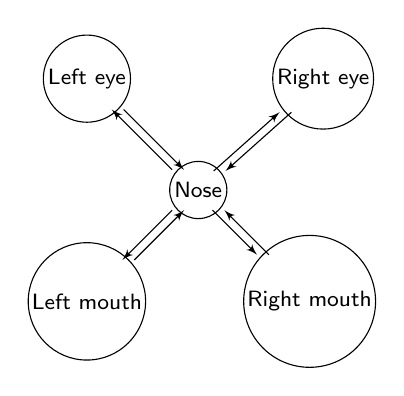
\begin{tikzpicture}[node distance=.5cm,auto,>=latex',font=\sffamily\footnotesize]
	        \node [circ] (a) {Right eye};
	        \node [circ] (b) [left of =a, node distance = 3cm] {Left eye};
	        \node [circ] (c) [below right of =b, node distance = 2cm] {Nose};
	        \node [circ] (d) [below left of =c, node distance = 2cm] {Left mouth};
	        \node [circ] (e) [below right of =c, node distance = 2cm] {Right mouth};
	        \draw[transform canvas={xshift=0.5ex},->] (a) -- (c);
	        \draw[transform canvas={xshift=-0.5ex},<-] (a) -- (c);
	       	\draw[transform canvas={xshift=0.5ex},->] (b) -- (c);
	        \draw[transform canvas={xshift=-0.5ex},<-] (b) -- (c);
	        \draw[transform canvas={xshift=0.5ex},->] (d) -- (c);
	        \draw[transform canvas={xshift=-0.5ex},<-] (d) -- (c);
	        \draw[transform canvas={xshift=0.5ex},->] (e) -- (c);
	        \draw[transform canvas={xshift=-0.5ex},<-] (e) -- (c);
	       
	    \end{tikzpicture}}
	\end{figure}
	We consider the probabilsitic model above to which we apply the max-product algorithm. Each leaf node \{Left eye, right eye, left mouth, right mouth\} (index $p$) passes a message to the root (index $r$) of the form:

	\[\begin{split}
	m_{p\to r}(X) & =\log\left(\max_{X_p}\Phi_p(X_p)\Psi_{p,r}(X_p,X_r)\right)\\
	& =\max_{X_p} \phi_p(X_p)+a\left(X_p(1)-X_r(1)\right)^2+b\left(X_p(1)-X_r(1)\right)+c\left(X_p(2)-X_r(2)\right)^2+d\left(X_p(2)-X_r(2)\right) + e 
	\end{split}\]
	where $\phi=\log\Phi, \psi=\log\Psi$  and $a,b,c,d$ and $e$ are parameters characterizing the distribution of the displacement vector $X_P-X_r$ assumed Gaussian.\\
	We have:
	\[\begin{cases}
	a=-\frac{1}{2\sigma_p(1)^2}\\
	b= \frac{\mu_p(1)}{\sigma_p(1)^2}\\
	c=-\frac{1}{2\sigma_p(2)^2}\\
	d =\frac{\mu_p(2)}{\sigma_p(2)^2}\\
	e = -\frac{\mu_p(1)^2}{2\sigma_p(1)^2}-\frac{\mu_p(2)^2}{2\sigma_p(2)^2}-\log(2\pi\sigma_1\sigma_2)
	\end{cases}\]
	The unary potentials are computed first with the provided SVM weights using SIFT features and then with an SVM learnt using the CNN2 features with the Alexnet architecture. 
	\subsection{Provided SVM model with SIFT}
		\begin{figure}[H]
		\centering
		\subfloat[Left eye]{\includegraphics[height=2cm]{dpm_sift/mess_pt1_3}}
		\hspace{10pt}\subfloat[Right eye]{\includegraphics[height=2cm]{dpm_sift/mess_pt2_3}}\\
		\subfloat[Left mouth]{\includegraphics[height=2cm]{dpm_sift/mess_pt3_3}}
		\hspace{10pt}\subfloat[Right mouth]{\includegraphics[height=2cm]{dpm_sift/mess_pt4_3}}
		\caption{Message passing : GDT vs Max-product (image 3)}
		\end{figure}
		At the root we collect the messages to compute the belief function $b(X) = \phi_r(X)+\sum_{i\neq r}m_{i\to r}(X)$
		\begin{figure}[H]
		\centering
		\includegraphics[width=10cm]{dpm_sift/belief_nose_3}
		\caption{Belief function at the root ($\equiv$ nose) - (image 3)}
		\end{figure}
		In a similar fashion, we send messages back to the parts:
		\[\begin{split}
		m_{r\to p}(X)  & = \log\left(\max_{X_r} \left[\Phi_r(X_r) \Psi_{r,p}(X_r,X_p)\prod_{k\in\mathcal N(r)\backslash p}M_{k\to r}(X_r)\right]\right)\\
		& = \max_{X_r}\left[\phi_r(X_r)+\psi_{r,p}(X_r,X_p)+\sum_{k\in\mathcal N(r)\backslash p}m_{k\to r}(X_r)\right]\\
		\end{split}\]
		\begin{figure}[H]
		\centering
		\subfloat[Left eye]{\includegraphics[width=2cm]{"dpm_sift/message_left eye_3"}}
		\hspace{5pt}\subfloat[Right eye]{\includegraphics[width=2cm]{"dpm_sift/message_right eye_3"}}
		\hspace{5pt}\subfloat[Left mouth]{\includegraphics[width=2cm]{"dpm_sift/message_left mouth_3"}}
		\hspace{5pt}\subfloat[Right mouth]{\includegraphics[width=2cm]{"dpm_sift/message_right mouth_3"}}

		\caption{Messages to the parts (image 3)}
		\end{figure}
	\newpage
	\subsection{Part 1' SVM model with CNN2}
	\textbf{Image 3:}
		\begin{figure}[H]
		\centering
		\subfloat[Left eye]{\includegraphics[height=1.8cm]{dpm_cnn2/mess_pt1_3}}
		\hspace{10pt}\subfloat[Right eye]{\includegraphics[height=1.8cm]{dpm_cnn2/mess_pt2_3}}\\
		\subfloat[Left mouth]{\includegraphics[height=1.8cm]{dpm_cnn2/mess_pt3_3}}
		\hspace{10pt}\subfloat[Right mouth]{\includegraphics[height=1.8cm]{dpm_cnn2/mess_pt4_3}}
		\caption{Message passing : GDT vs Max-product (image 3)}
		\end{figure}
		\begin{figure}[H]
		\centering
		\includegraphics[width=8cm]{dpm_cnn2/belief_nose_3}
		\caption{Belief function at the root ($\equiv$ nose) - (image 3)}
		\end{figure}
		\begin{figure}[H]
		\centering
		\subfloat[Left eye]{\includegraphics[width=2cm]{"dpm_cnn2/message_left eye_3"}}
		\hspace{5pt}\subfloat[Right eye]{\includegraphics[width=2cm]{"dpm_cnn2/message_right eye_3"}}
		\hspace{5pt}\subfloat[Left mouth]{\includegraphics[width=2cm]{"dpm_cnn2/message_left mouth_3"}}
		\hspace{5pt}\subfloat[Right mouth]{\includegraphics[width=2cm]{"dpm_cnn2/message_right mouth_3"}}

		\caption{Messages to the parts (image 3)}
		\end{figure}
	\textbf{Image 231:}
		\begin{figure}[H]
		\centering
		\subfloat[Left eye]{\includegraphics[height=1.8cm]{dpm_cnn2/mess_pt1_231}}
		\hspace{10pt}\subfloat[Right eye]{\includegraphics[height=1.8cm]{dpm_cnn2/mess_pt2_231}}\\
		\subfloat[Left mouth]{\includegraphics[height=1.8cm]{dpm_cnn2/mess_pt3_231}}
		\hspace{10pt}\subfloat[Right mouth]{\includegraphics[height=1.8cm]{dpm_cnn2/mess_pt4_231}}
		\caption{Message passing : GDT vs Max-product (image 231)}
		\end{figure}
		\begin{figure}[H]
		\centering
		\includegraphics[width=8cm]{dpm_cnn2/belief_nose_231}
		\caption{Belief function at the root ($\equiv$ nose) - (image 231)}
		\end{figure}
		\begin{figure}[H]
		\centering
		\subfloat[Left eye]{\includegraphics[width=2cm]{"dpm_cnn2/message_left eye_231"}}
		\hspace{5pt}\subfloat[Right eye]{\includegraphics[width=2cm]{"dpm_cnn2/message_right eye_231"}}
		\hspace{5pt}\subfloat[Left mouth]{\includegraphics[width=2cm]{"dpm_cnn2/message_left mouth_231"}}
		\hspace{5pt}\subfloat[Right mouth]{\includegraphics[width=2cm]{"dpm_cnn2/message_right mouth_231"}}

		\caption{Messages to the parts (image 231)}
		\end{figure}

	\textbf{Image 507:}
		\begin{figure}[H]
		\centering
		\subfloat[Left eye]{\includegraphics[height=1.8cm]{dpm_cnn2/mess_pt1_507}}
		\hspace{10pt}\subfloat[Right eye]{\includegraphics[height=1.8cm]{dpm_cnn2/mess_pt2_507}}\\
		\subfloat[Left mouth]{\includegraphics[height=1.8cm]{dpm_cnn2/mess_pt3_507}}
		\hspace{10pt}\subfloat[Right mouth]{\includegraphics[height=1.8cm]{dpm_cnn2/mess_pt4_507}}
		\caption{Message passing : GDT vs Max-product (image 507)}
		\end{figure}
		\begin{figure}[H]
		\centering
		\includegraphics[width=8cm]{dpm_cnn2/belief_nose_507}
		\caption{Belief function at the root ($\equiv$ nose) - (image 507)}
		\end{figure}
		\begin{figure}[H]
		\centering
		\subfloat[Left eye]{\includegraphics[width=2cm]{"dpm_cnn2/message_left eye_507"}}
		\hspace{5pt}\subfloat[Right eye]{\includegraphics[width=2cm]{"dpm_cnn2/message_right eye_507"}}
		\hspace{5pt}\subfloat[Left mouth]{\includegraphics[width=2cm]{"dpm_cnn2/message_left mouth_507"}}
		\hspace{5pt}\subfloat[Right mouth]{\includegraphics[width=2cm]{"dpm_cnn2/message_right mouth_507"}}

		\caption{Messages to the parts (image 507)}
		\end{figure}

\section{Multi-scale detection , non-maximum suppression, benchmarking}	
	
	We perform feature extraction with the previously trained SVM on the CNN2 features then compute the unary scoes and run GDT to compute the belief at the root at different scales $[2^{-1}, 2^{-0.5}, 1, 2^{0.5}, 2]$. The input image remains unnormalized i.e. we do not correct the distance between the eyes. The candidate roots are selected when the belief is above a selection threshold and the remaining parts are located using the $ix$ and $iy$ maps outputted by GDT given the root location.
	\begin{figure}[H]
	\centering
	\includegraphics[width=3cm]{"part3/thp05/bbox_left eye_3"}
	\includegraphics[width=3cm]{"part3/thp05/bbox_right eye_3"}
	\includegraphics[width=5cm]{"part3/thp05/bbox_nose_3"}
	\includegraphics[width=3cm]{"part3/thp05/bbox_left mouth_3"}
	\includegraphics[width=3cm]{"part3/thp05/bbox_right mouth_3"}
	\caption{Threshold = 0.5 - image 3} 
	\end{figure}
	\begin{figure}[H]
	\centering
	\includegraphics[width=3cm]{"part3/thp05/bbox_left eye_231"}
	\includegraphics[width=3cm]{"part3/thp05/bbox_right eye_231"}
	\includegraphics[width=5cm]{"part3/thp05/bbox_nose_231"}
	\includegraphics[width=3cm]{"part3/thp05/bbox_left mouth_231"}
	\includegraphics[width=3cm]{"part3/thp05/bbox_right mouth_231"}
	\caption{Threshold = 0.5 - image 231} 
	\end{figure}
	\begin{figure}[H]
	\centering
	\includegraphics[width=3cm]{"part3/thp05/bbox_left eye_507"}
	\includegraphics[width=3cm]{"part3/thp05/bbox_right eye_507"}
	\includegraphics[width=5cm]{"part3/thp05/bbox_nose_507"}
	\includegraphics[width=3cm]{"part3/thp05/bbox_left mouth_507"}
	\includegraphics[width=3cm]{"part3/thp05/bbox_right mouth_507"}
	\caption{Threshold = 0.5 - image 507} 
	\end{figure}

	With a lower threshold we can suggest more locations:
	\begin{figure}[H]
	\centering
	\subfloat[image 3]{\includegraphics[width=4cm]{"part3/thn05/bbox_nose_3"}}
	\hspace{3pt}\subfloat[image 231]{\includegraphics[width=4cm]{"part3/thn05/bbox_nose_231"}}
	\hspace{3pt}\subfloat[image 507]{\includegraphics[width=4cm]{"part3/thn05/bbox_nose_507"}}
	\end{figure}
	\begin{figure}[H]
	\centering
	\subfloat[image 3]{\includegraphics[width=4cm]{"part3/thn05/bbox_left mouth_3"}}
	\hspace{3pt}\subfloat[image 231]{\includegraphics[width=4cm]{"part3/thn05/bbox_left mouth_231"}}
	\hspace{3pt}\subfloat[image 507]{\includegraphics[width=4cm]{"part3/thn05/bbox_left mouth_507"}}
	\caption{Threshold = -0.5} 
	\end{figure}

	To filter the suggested boxes we apply non-maximum suppression with an overlap threshold of 0.7
	\begin{figure}[H]
	\centering
	\subfloat[image 3]{\includegraphics[width=4cm]{"part3/thn05/nms_bbox_nose_3"}}
	\hspace{3pt}\subfloat[image 231]{\includegraphics[width=4cm]{"part3/thn05/nms_bbox_nose_231"}}
	\hspace{3pt}\subfloat[image 507]{\includegraphics[width=4cm]{"part3/thn05/nms_bbox_nose_507"}}\\
	\subfloat[image 3]{\includegraphics[width=4cm]{"part3/thn05/nms_bbox_left mouth_3"}}
	\hspace{3pt}\subfloat[image 231]{\includegraphics[width=4cm]{"part3/thn05/nms_bbox_left mouth_231"}}
	\hspace{3pt}\subfloat[image 507]{\includegraphics[width=4cm]{"part3/thn05/nms_bbox_left mouth_507"}}

	
	\caption{NMS - box selection thresold  -0.5  - box overlap threshold 0.7}
	\end{figure}
\end{document}